\section{Tafel ronde 3: raadsel ronde}
\begin{questions}
\question[4] {\begin{flushleft}
{\large Raadsel 1: Twenty-one}
\end{flushleft}
\begin{flushleft}
Dit raadsel komt van de thuisstad van Tibo (cultuur home Astrid). In Koksijde staan er veel wetgevingen op hoogte bouw, dus is er maar één echt super hoog gebouw: de Twenty-one. Rara-ra, het gebouw heeft 21 verdiepen. Nu woont de beste vriend van Freddy op de 21ste verdieping. Elke dag als het mooi weer is neemt hij de lift naar beneden en de trap naar boven. Echter wanneer het slecht weer is neemt hij de lift naar beneden en ook de lift naar boven.
\linebreak
De vraag is, hoe komt dit? Waarom neemt hij niet altijd de lift?
\linebreak
\end{flushleft}
}
\it Hint: op slechte dagen neemt hij een paraplu mee!
\fillwithlines{\stretch{1}}
%raadsel 2
\question[2]{\begin{flushleft}
{\large Raadsel 2: Vogel}
\end{flushleft} Maak een vogel door 2 rechte strepen te plaatsen.\center
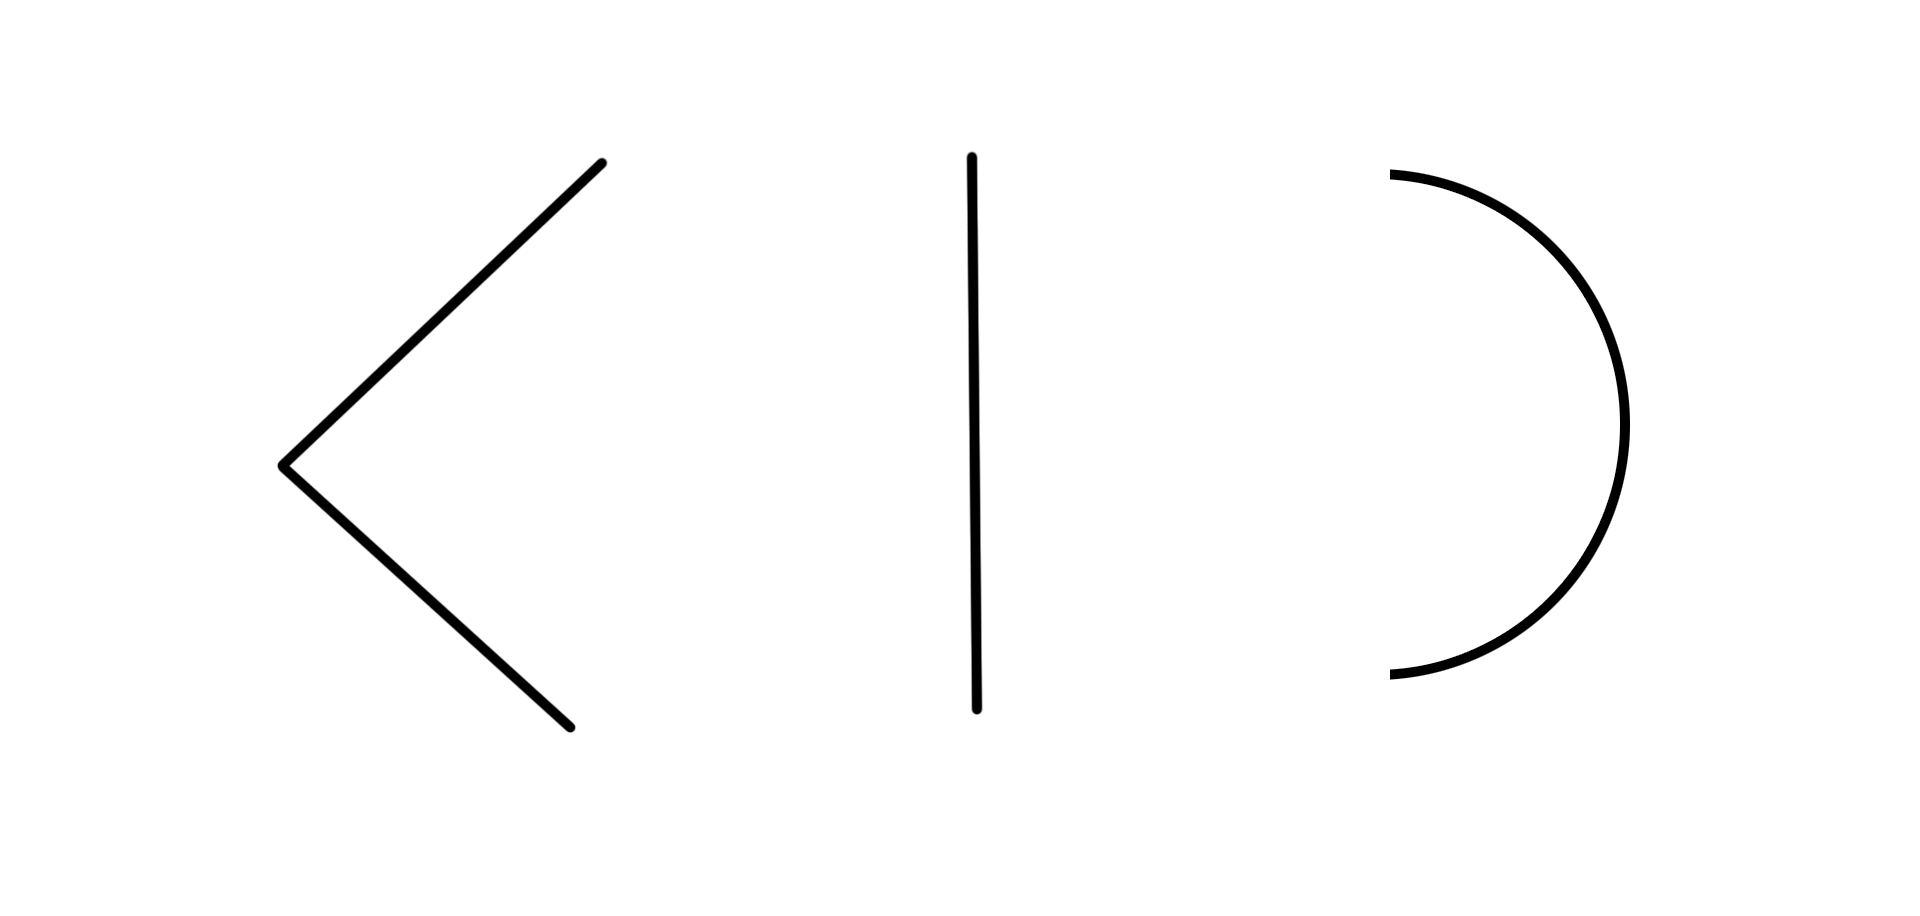
\includegraphics[scale=1]{kip}}
\newpage
\question[2]{\begin{flushleft}
{\large Raadsel 3: converteer het symbool naar een decimaal getal.}
\end{flushleft}
\begin{center}
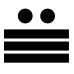
\includegraphics[scale=0.4]{76}
\end{center}
\fillwithlines{2em}
}


\question[2] {\begin{flushleft}
{\large Raadsel 4: Ontcijfer}
\end{flushleft}
\begin{flushleft}
Ontcijfer deze boodschap!
\end{flushleft}
\begin{center}
Oleacahoydnebp xef 4
\end{center}
\it Hint! Kijk naar het nummer van het raadsel!
\fillwithlines{3em}
}

\newpage
\question[2] {\begin{flushleft}
{\large Raadsel 4: Symbolen}
\end{flushleft}
Bepaal de volgende symbolen (mintens 2 aanvullen ,maar maximum 5).
\center
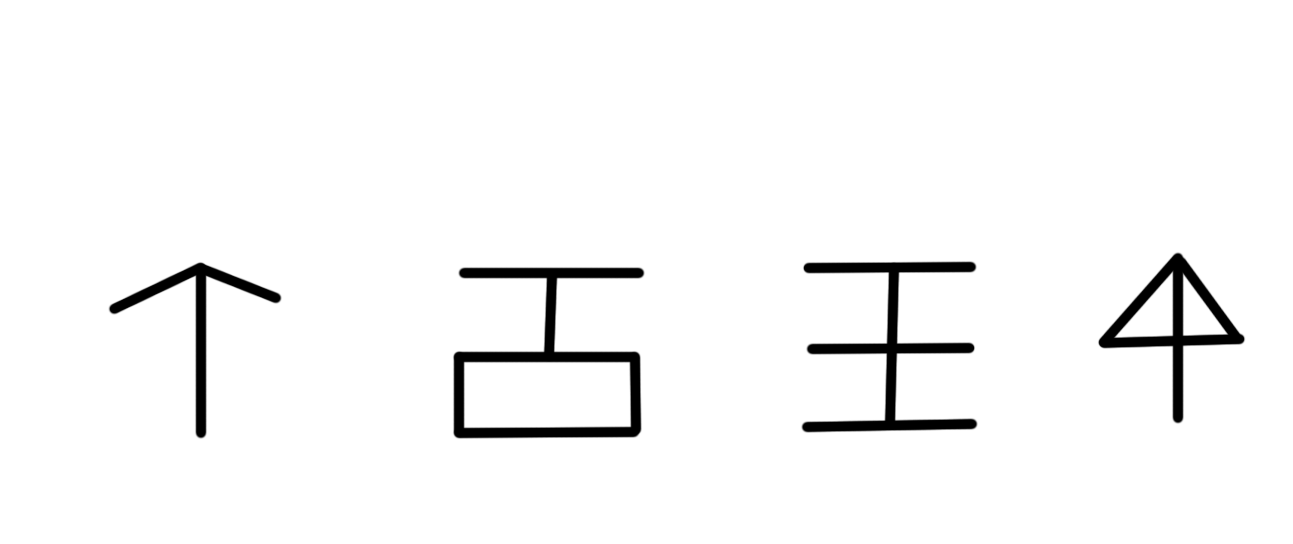
\includegraphics[scale=1]{symbolen}
}



\question[2]{\begin{flushleft}
{\large Raadsel 6: Freddy probeert 8 konoginnnen op een schaakbord te zetten, zonder dat ze elkaar in de weg staan. Een koningin kan elke kant uit, dus ze kan horizontaal, verticaal en diagonaal bewegen. }
\end{flushleft}
\begin{center}

\includegraphics[scale=0.03]{schaakbord2}
\end{center}
\newpage
\question[4]{
Er zijn 4 verschillende dozen gegeven, telkens met bijhorend opschrift:

\vspace{0.2cm}

Doos A: \framebox[0.4\textwidth][l]{Het punt zit niet in doos B}

\vspace{0.2cm}

Doos B: \framebox[0.4\textwidth][l]{Het punt zit niet in doos C}

\vspace{0.2cm}

Doos C: \framebox[0.4\textwidth][l]{Het punt zit in doos D}

\vspace{0.2cm}

Doos D: \framebox[0.4\textwidth][l]{Het punt zit in doos A}
\vspace{0.2cm}

Er is maar één doos die de waarheid spreekt.
Je mag maar 1 doos kiezen en openen! 

\textbf{Er is een wiskundige manier voor deze vraag! men kan dit formaliseren met proposities en eventueel verzamelingenleer.}

{\em Opmerking:} om alle punten te krijgen moet je ook proposities geven!}
}
\newpage
\question[2]{
Er rijd een zwarte auto op een zwarte baan, de gebouwen zijn zwart en de bewoners hebben hun zwarte gordijnen gesloten. De autolichten en straatverlichting zijn gedooft. De auto stopt en laat de zwarte kat oversteken. Hoe komt het dat de autobestuurder de zwarte kat zag?

\fillwithlines{\stretch{1}}
}
\end{questions}
\begin{table}[!b]
\centering
\begin{tabular}{|l|l|l|l|l|l|l|l|l|l|l|}
\hline
Vraag       & 1 & 2 & 3 & 4 & 5 & 6 & 7 & 8 \\ \hline
max. punten & 4 & 2 & 2 & 2 & 2 & 2 & 4 & 2 \\ \hline
score       &   &   &   &   &   &   &   &   \\ \hline
\end{tabular}
\end{table}